\chapter{迁移学习的可学习性}
\label{chap:transfer-learning-theory}

一个邮件分类器在过去几个月的邮件上取得了较小的经验风险。此前各章讨论了怎样控制假设空间或学习算法，使这个结果能够说明它在同一数据分布下的期望风险。部署到新的月份后，问题又多了一层：新月份的邮件可能具有不同的输入分布，同一输入对应的标签也可能改变。即使源域样本已经足够多，原有的泛化保证也未必适用于目标域。

迁移学习理论需要同时回答两个问题。已有观测是否包含判断目标域标签所需的信息；如果包含，需要多少样本才能把这些信息转化为可靠的预测。前一个问题取决于源域与目标域保留了什么联系，后一个问题还取决于假设空间和学习算法的复杂度。VC维、参数范数、参数分布和算法稳定性仍然有用，但它们必须与跨域条件结合，才能支持目标域期望风险的保证。

为把信息是否足够与有限样本能否估计分开，第~\ref{sec:transfer-learning-setting}节先固定
数据、评价目标与允许的分布变化；其中的反例给出后续保证必须跨过的可识别性门槛。
目标域输入可用时，第~\ref{sec:domain-adaptation}节把跨域风险连接与复杂度或稳定性
控制结合起来。训练阶段连目标域输入也不可用时，第~\ref{sec:domain-generalization}节
分别在共享标签机制和环境抽样两类条件下建立保证，并比较逐目标域与环境平均保证各自
能够支持的结论。

\section{迁移学习的学习问题}
\label{sec:transfer-learning-setting}

\subsection{数据与评价目标}
\label{sec:adaptation-generalization-settings}

沿用第~\ref{sec:transfer-learning}节的术语，迁移学习利用已有领域或任务中的信息帮助新的
学习问题。本章只研究输入空间$X$与标签空间$Y$保持相同、联合分布发生变化的情形，并把
一个域形式化为$X\times Y$上的联合分布。跨任务迁移以及输入、标签空间变化不在本章的
形式结论范围内。提供已有数据的环境仍称为源域，最终需要作出预测的环境称为目标域。
例如，过去月份的邮件来自源域，即将处理的新月份邮件来自目标域。

记源域与目标域的联合分布分别为$\mathcal P_S$和$\mathcal P_T$，它们都定义在$X\times Y$上。固定假设空间$\mathcal H$与取值在$[0,1]$中的预测级损失
$\ell_{\mathrm{pred}}(\widehat y,y)$，并令
$\ell_h(x,y)=\ell_{\mathrm{pred}}(h(x),y)$。同一个假设$h$在两域上的期望风险分别为
\begin{equation}
 R_S(h)=\mathbb E_{\mathcal P_S}\ell_h(x,y),\qquad
 R_T(h)=\mathbb E_{\mathcal P_T}\ell_h(x,y).
 \label{eq:transfer-population-risks}
\end{equation}
这里$R_S$与$R_T$的下标分别标明源域与目标域；有帽号的$\hat R$才表示经验风险。
后文用$\mathcal P_D^X$表示域$D$的输入边缘分布，以免把域的标记与输入的标记混淆。
本章默认损失及涉及的上确界具有所需的可测性，各随机抽样过程均定义良好。

目标域期望风险$R_T(h)$才是部署时要控制的量。其比较基准通常为
$R_{T,\mathcal H}^{\star}=\inf_{h\in\mathcal H}R_T(h)$，即同一假设空间在目标域
能够达到的最低期望风险。差值$R_T(h)-R_{T,\mathcal H}^{\star}$称为
\term{目标域超额期望风险}（target-domain excess risk）。这个基准可能大于零；
可学习性要求学到接近基准的假设，并不要求消除输入信息不足带来的全部错误。

理论结论还取决于算法能够观察什么。\term{领域自适应}（domain adaptation）允许在学习阶段使用目标域样本。本章重点分析无监督领域自适应：算法收到带标签的源域样本$S_S$与无标签的目标域样本$U_T$，其中
\[
 S_S\sim\mathcal P_S^{n_S},\qquad
 U_T\sim(\mathcal P_T^X)^{n_T},
\]
两批样本相互独立，$\mathcal P_T^X$表示只保留输入的目标域边缘分布。若能够取得足够多的目标域标签，直接在目标域应用前几章的PAC理论便可得到学习保证；迁移理论进一步研究源域信息能否减少对目标域标签的需求。

领域泛化（domain generalization）在训练与模型选择阶段不使用目标域样本。算法只能使用若干训练环境的带标签样本，再把学到的假设用于未见环境。预测时读入一个新输入是必要的；这里排除的是利用目标域样本更新假设或选择模型。缺少目标域数据后，需要更明确地规定哪些新环境属于允许的评价范围。若部署阶段根据一批目标输入更新参数、归一化统计量或模型选择结果，就进入第~\ref{sec:transfer-learning}节所说的测试时适应；此时输出对象是适应算法，抽样时序、批次依赖和评价基准都需重新定义，本章的固定输出领域泛化定理不能直接套用。

为了区分算法可见的信息、评价对象和概率来源，还需把这两类问题细分为三种设定。
领域自适应固定一组源域与目标域，算法观察源域带标签样本$S_S$和目标域无标签输入
$U_T$，输出用于该目标域的假设。评价对象是目标域风险$R_T$，比较基准是
$R_{T,\mathcal H}^{\star}$，保证中的概率来自两批样本和算法随机性。

\term{逐目标域领域泛化}（target-wise domain generalization）固定训练域组，并把一个
允许的目标域作为外层量词给定。算法只能观察训练域的带标签样本，输出不能针对该目标域
重新选择；每个目标域上的评价风险和比较基准仍分别是$R_T$与
$R_{T,\mathcal H}^{\star}$。此时保证中的概率来自训练域样本和算法随机性，目标域本身
不在该概率中平均。

\term{环境平均领域泛化}（environment-average domain generalization）则先规定环境分布
$\mathcal Q$，从中抽取$K$个训练环境，并在每个环境内取得一个数据块。算法输出用于未来
随机环境的共同假设，评价风险为
$R_{\mathcal Q}(h)=\mathbb E_{\mathcal P\sim\mathcal Q}R_{\mathcal P}(h)$，比较基准是
$\inf_{h\in\mathcal H}R_{\mathcal Q}(h)$。相应概率同时包含环境抽样、环境内抽样和算法
随机性。三种设定沿用同一损失、输出范围、可测性和计算层次，但分布对象、可见信息、
比较基准与概率来源不同。

\subsection{分布偏移与可识别性}
\label{sec:distribution-shift}

源域与目标域的联系可以通过联合分布的分解来描述。若两个域中同一输入的标签规律不变，源域标签仍能提供相关信息；若标签规律也可以任意改变，再多源域样本也不能说明目标域应当如何分类。下面的设定指出哪些部分允许变化，哪些部分被假定保留。为避免在源域从未出现的输入上比较任意选取的条件概率版本，协变量偏移还需与后文的覆盖条件结合使用。

\begin{definition}[协变量偏移]
\label{def:covariate-shift}
若存在一个条件标签分布$\mathsf K(\mathrm dy\mid x)$，使得
\[
 \mathcal P_D(\mathrm dx,\mathrm dy)
 =\mathcal P_D^X(\mathrm dx)\mathsf K(\mathrm dy\mid x),
 \qquad D\in\{S,T\},
\]
则称两域满足协变量偏移设定。该设定允许$\mathcal P_S^X$与$\mathcal P_T^X$不同。
\end{definition}

协变量偏移（covariate shift）保留给定输入后的标签分布。例如，目标域的长邮件更多，但在长邮件内部、短邮件内部，诈骗比例分别保持不变。若一个分类器在长邮件上更容易出错，长邮件比例增加仍会提高它的目标域期望风险；条件标签分布不变并不意味着两个期望风险相同。

\begin{definition}[标签偏移]
\label{def:label-shift}
若存在条件输入分布$\mathsf K(\mathrm dx\mid y)$，使得
\[
 \mathcal P_D(\mathrm dx,\mathrm dy)
 =\mathcal P_D^Y(\mathrm dy)\mathsf K(\mathrm dx\mid y),
 \qquad D\in\{S,T\},
\]
则称两域满足标签偏移设定。该设定允许$\mathcal P_S^Y$与$\mathcal P_T^Y$不同。
\end{definition}

标签偏移（label shift）保留每个类别内部的输入分布。例如，诈骗邮件的总体比例增加，但诈骗邮件内部的特征分布不变，正常邮件内部的特征分布也不变。类别比例的改变通常会同时改变给定输入后的类别概率，所以标签偏移与协变量偏移是不同的假设。

\term{概念偏移}（concept shift）指给定输入后的标签分布发生变化，也称条件偏移。例如，源域长邮件中的诈骗比例为0.1，目标域却变为0.4，即使长邮件本身的出现频率不变，源域标签也不能直接代表目标域标签。本章比较条件分布时，均在两域共同覆盖的输入区域上理解这种变化；若目标域出现源域完全未覆盖的输入，还存在额外的信息缺失。

这三种设定不是互斥分类。标签偏移虽然保持$\mathcal P(x\mid y)$，类别比例变化通常仍会
改变$\mathcal P(y\mid x)$，因而也呈现后验条件分布变化；“概念偏移”在这里描述被改变的
条件机制，不表示它与标签偏移构成互斥的剩余类别。图~\ref{fig:learning-distribution-shift}
对比了这些变化发生的位置。图中的区别说明跨域假设保留了哪一部分信息，并不单独构成
可学习性结论。例如，协变量偏移没有规定目标域是否包含源域从未出现的输入；标签偏移也
没有保证仅凭无标签输入就能确定新的类别比例。
\begin{figure*}[htbp]
  \centering
  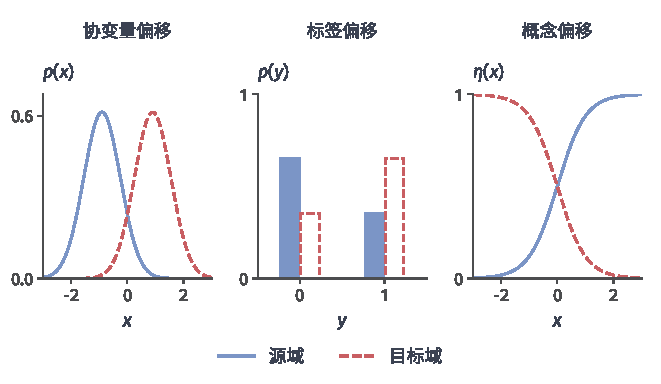
\includegraphics[width=164.600mm]{figures/02-foundations/02-learning-theory/matplotlib/learning-theory-distribution-shift/figure.pdf}
  \caption{分布偏移改变联合分布的不同组成部分。实线表示源域，虚线表示目标域；密度、类别比例和条件概率均为规范化的教学构造，不表示实测频率。协变量偏移允许输入分布改变，标签偏移允许类别比例改变，概念偏移则改变给定输入后的标签分布，图中$\eta(x)=\mathbb P(y=1\mid x)$。这些设定还需与覆盖条件或其他可识别条件结合，才能支持迁移保证。}
 \label{fig:learning-distribution-shift}
\end{figure*}

输入密度如何变化，与目标输入能否在源域中出现，是两个问题。
图~\ref{fig:learning-support-coverage}用同一坐标尺度比较三种覆盖程度。
目标域的支持完全位于源域支持内时，每个目标区域原则上都能获得源域观测；
部分或几乎全部目标区域没有源域概率时，在这些区域重复增加源域样本也不能补上标签信息。
即使完全覆盖，源域概率过小仍会造成后文密度比过大的困难。

\begin{figure*}[!htb]
  \centering
  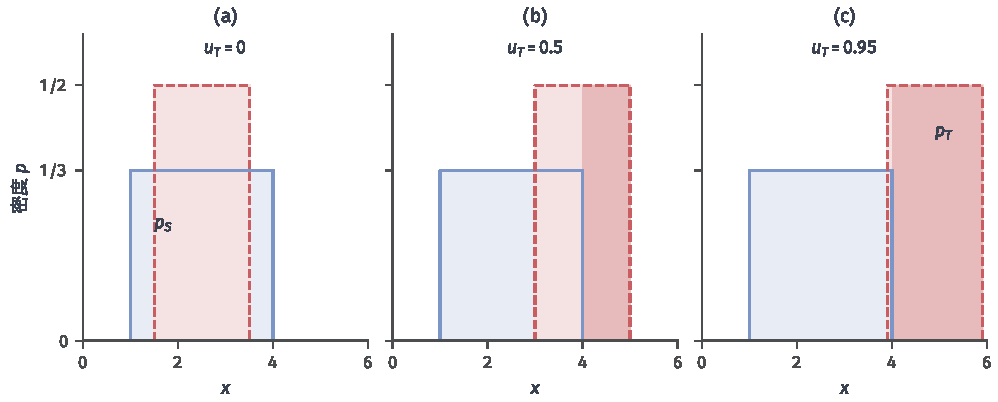
\includegraphics[width=164.600mm]{figures/02-foundations/02-learning-theory/matplotlib/learning-theory-support-coverage/figure.pdf}
  \caption{同尺度的三种支持覆盖。源密度均为$[1,4]$上的$1/3$，目标密度均为长度2区间上的$1/2$；(a)、(b)、(c)的目标支持依次为$[1.5,3.5]$、$[3,5]$、$[3.9,5.9]$。深色区域没有源密度，其目标概率$u_T=\mathbb P_T\{p_S(X)=0\}$依次为0、0.5、0.95。实线、虚线与底色共同区分源域、目标域；只有(a)满足覆盖条件$p_T(x)>0\Rightarrow p_S(x)>0$。密度为规范化教学构造，不是实验分布。}
 \label{fig:learning-support-coverage}
\end{figure*}
\FloatBarrier

图~\ref{fig:learning-alignment-counterexample}给出更直接的边界：即使输入分布相同，两种相反的目标标签规律也能产生相同的可观察数据。仅使表示或输入分布接近，不能自动建立迁移保证。

这里需要区分“样本还不够多”与“现有类型的数据没有提供答案”。第一卷的
\BookDefinitionRef{def:statistics-identifiability}{可识别性定义}
要求观测分布相同的两个允许机制给出相同目标泛函。本章把目标泛函取为目标域标签核、
目标域最优决策或相应风险；如果两种可能机制产生完全相同的可观察数据，却给出不同目标，
算法就无法判断当前是哪一种规律。这就是本章所说的\term{可识别性}（identifiability）
问题。下面的定理把这种信息缺失与假设空间大小分开。

\begin{figure*}[!htb]
  \centering
  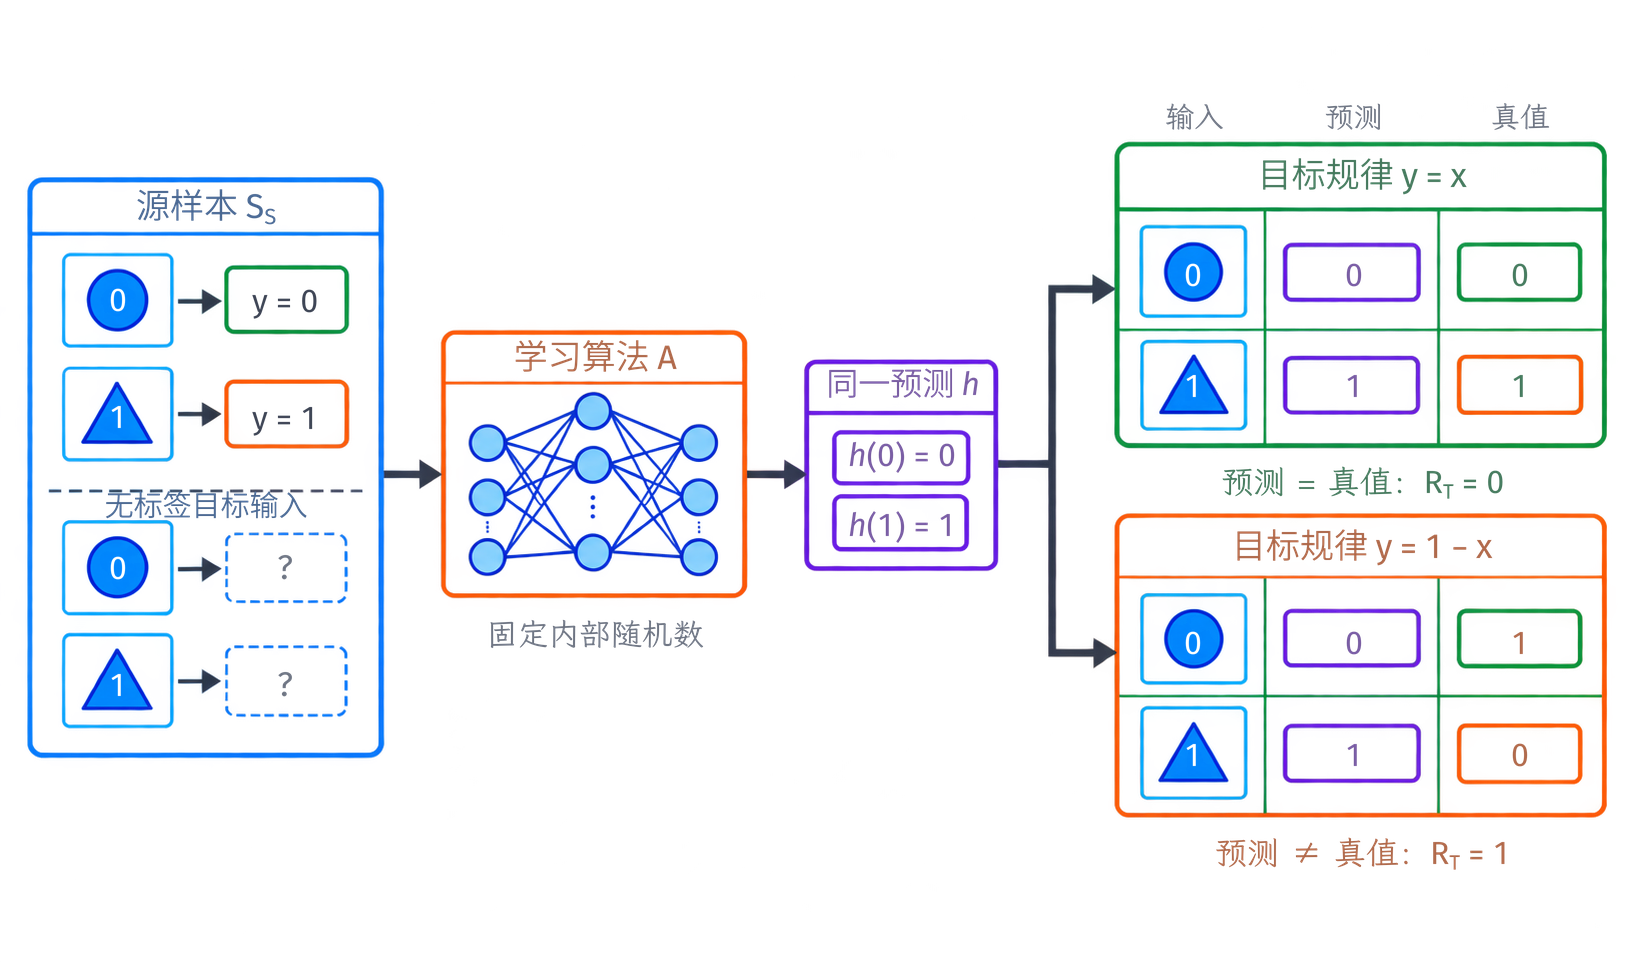
\includegraphics[width=164.600mm]{figures/02-foundations/02-learning-theory/generated/learning-theory-alignment-counterexample/figure.png}
  \caption{相同可观察数据不能区分两种目标规律。两域都以概率$1/2$产生输入0或1，源标签为$y=x$。算法只收到左侧带标签源样本和无标签目标输入，目标标签并未提供；右侧两种可能分别取$y=x$与$y=1-x$。固定算法内部随机数后，两种情形必得到同一输出。图中以$h(x)=x$为例，两张表逐点对照同一预测与隐藏标签：零一损失下，源风险为0，两种目标风险分别为0、1。任意二分类输出在这两种目标规律下的风险之和为1。输入完全对齐仍未提供选择目标规律的证据，还需目标标签或连接两域标签规律的额外条件。}
  \label{fig:learning-alignment-counterexample}
\end{figure*}
\FloatBarrier


\begin{theorem}[缺少覆盖时的不可学习性]
\label{thm:transfer-nonidentifiability}
采用二分类零一损失。令$X=\{a,b\}$、$Y=\{0,1\}$，且
$\mathcal H=\{h_0,h_1\}$满足
\[
 h_0(a)=h_1(a)=0,\qquad h_0(b)=0,\quad h_1(b)=1.
\]
源域恒产生$(a,0)$，目标域输入恒为$b$。允许的两个目标域分别令$b$的标签恒为0或恒为1。
对任意只使用带标签源域样本与无标签目标域样本、输出属于$\mathcal H$的可能随机化
学习算法$A$，无论两类样本量多大，总有一个允许的目标域满足
\[
 \mathbb P_{S_S,U_T,A}\!\left(
 R_T(A(S_S,U_T))>\tfrac14
 \right)\geq\tfrac12.
\]
这里概率包含抽样与算法内部的随机性。两个设定各自都存在源域与目标域期望风险同时为零的假设。
\end{theorem}
\begin{proof}
两种设定中，算法收到的全部源域样本都是$(a,0)$，全部目标域输入都是$b$，因此
输入数据的分布完全相同。设算法输出$h_1$的概率为$p$；这个概率只可能来自算法内部
随机性，且在两个设定中相同。目标标签为0时，算法以概率$p$输出$h_1$，其目标域
零一风险为1；目标标签为1时，算法以概率$1-p$输出$h_0$，其目标域零一风险也为1。
两者至少有一个不小于$1/2$。标签为0的设定中$h_0$在两域均无错误，标签为1的设定中
$h_1$在两域均无错误，故失败并非假设空间缺少合适的假设。
\end{proof}

这个假设空间只有两个假设，VC维为1。减少参数数量、限制参数大小，甚至允许无限源域样本，都不能确定$b$的目标标签。反例也符合共享条件标签机制的描述：每种设定都可把同一标签规律定义在$\{a,b\}$上，但源域永远不提供$b$的信息。迁移学习的不可学习性研究因此需要同时检查分布联系与可观察数据，而不能只检查假设空间复杂度\scite{bendavid2010impossibility}。

\subsection{迁移学习的PAC要求}
\label{sec:transfer-pac-setting}

前面的反例要求我们明确“对哪些分布保证学习成功”。记$\mathfrak P_{\mathrm{DA}}$为允许的源域、目标域联合分布对组成的集合。共享条件标签机制、输入覆盖程度以及算法已知的分布信息，都应当写入问题设定。改变这些条件，可能改变同一个假设空间的可学习性。

\begin{definition}[相对于分布族的领域自适应PAC可学习性]
\label{def:adaptation-pac-learnability}
固定$\mathcal H$、损失函数$\ell$及允许的分布对集合$\mathfrak P_{\mathrm{DA}}$。若存在取值于$\mathcal H$的学习算法$A$与有限的样本量函数$m_S,m_T$，使得对任意$\varepsilon,\delta\in(0,1)$、任意$(\mathcal P_S,\mathcal P_T)\in\mathfrak P_{\mathrm{DA}}$，以及$n_S\geq m_S(\varepsilon,\delta)$、$n_T\geq m_T(\varepsilon,\delta)$，都有
\[
 \mathbb P_{S_S,U_T,A}\!\left(
 R_T(A(S_S,U_T))-R_{T,\mathcal H}^{\star}\leq\varepsilon
 \right)\geq1-\delta,
\]
则称$\mathcal H$在该设定下是领域自适应PAC可学习的。样本量函数可以依赖$\mathcal H$及$\mathfrak P_{\mathrm{DA}}$的统一参数，但不能依赖其中未知的具体分布对。
\end{definition}

这里采用输出属于$\mathcal H$的学习要求，并允许不可知设定，即$R_{T,\mathcal H}^{\star}$不必为零。若问题还给出已知的密度比等辅助信息，应把这些信息作为算法的额外输入。定义只要求统计上的可学习性，寻找满足要求的假设是否能够高效完成，是另一个问题。

\begin{definition}[逐目标域领域泛化PAC可学习性]
\label{def:targetwise-domain-generalization-pac}
设$\mathfrak P_{\mathrm{DG}}$是允许训练域组$\mathcal D=(\mathcal P_1,\ldots,\mathcal P_K)$的集合，并为每个$\mathcal D$指定允许目标域集合$\mathcal T(\mathcal D)$。记训练域均匀混合为$\overline{\mathcal P}_{\mathcal D}=K^{-1}\sum_{e=1}^K\mathcal P_e$。若存在取值于$\mathcal H$的算法$A$和有限样本量函数$m$，使对任意$\varepsilon,\delta\in(0,1)$、任意$\mathcal D\in\mathfrak P_{\mathrm{DG}}$、任意固定的$\mathcal P_T\in\mathcal T(\mathcal D)$及任意$n\geq m(\varepsilon,\delta)$，都有
\[
 \mathbb P_{S\sim\overline{\mathcal P}_{\mathcal D}^{\,n},A}\!\left(
 R_T(A(S))-R_{T,\mathcal H}^{\star}\leq\varepsilon
 \right)\geq1-\delta,
\]
则称$\mathcal H$在该设定下是\term{逐目标域领域泛化}（target-wise domain generalization）PAC可学习的。算法在训练和模型选择时不接收目标域样本；目标域由概率之外的全称量词固定。
\end{definition}

这个定义要求同一个算法与样本量门槛适用于每个允许目标域，但每个目标域可以对应不同的高概率事件。若一个结论用同一个训练样本事件同时控制全部允许目标域，它比逐目标域定义要求更强。

\begin{definition}[环境平均领域泛化PAC可学习性]
\label{def:environment-average-domain-generalization-pac}
设$\mathfrak M$是允许的环境分布族，其中每个$\mathcal Q\in\mathfrak M$都是$Z$上概率分布的分布。训练时先独立抽取$\mathcal P_1,\ldots,\mathcal P_K\sim\mathcal Q$，再从每个环境抽取数据块$D_e\sim\mathcal P_e^n$，算法只接收$\mathcal S=(D_1,\ldots,D_K)$。定义
\[
 R_{\mathcal Q}(h)=\mathbb E_{\mathcal P\sim\mathcal Q}R_{\mathcal P}(h).
\]
若存在取值于$\mathcal H$的算法$A$以及有限的环境数门槛$k_0$和总观测数门槛$m_0$，使对任意$\varepsilon,\delta\in(0,1)$、任意$\mathcal Q\in\mathfrak M$，只要$K\geq k_0(\varepsilon,\delta)$且$Kn\geq m_0(\varepsilon,\delta)$，就有
\[
 \mathbb P_{\mathcal P_1,\ldots,\mathcal P_K,D_1,\ldots,D_K,A}\!\left(
 R_{\mathcal Q}(A(\mathcal S))-\inf_{h\in\mathcal H}R_{\mathcal Q}(h)
 \leq\varepsilon
 \right)\geq1-\delta,
\]
则称$\mathcal H$在该设定下是\term{环境平均领域泛化}（environment-average domain generalization）PAC可学习的。
\end{definition}

环境平均保证的概率包含训练环境、环境内观测和算法随机性；未来环境已经在$R_{\mathcal Q}$中取平均。比较基准是同一个假设在环境分布上的最低平均风险，而不是允许每个环境分别选择最优假设后再取平均。只有当相应超额期望风险能够随两层样本量增加而任意减小时，才能得到定义~\ref{def:environment-average-domain-generalization-pac}中的PAC可学习性。

三种设定都要求先说明允许的分布族。一个上界若始终保留正的分布偏移项，仍可揭示目标域表现受哪些因素影响，却不能直接证明任意精度的PAC学习。下面的定理将分别注明它支持领域自适应、逐目标域领域泛化还是环境平均领域泛化。

\section{领域自适应的可学习性}
\label{sec:domain-adaptation}

无标签目标域样本能够帮助估计目标输入分布，却不直接提供目标标签。因此，领域自适应的论证需要完成两步：先说明源域风险与可观察的目标域输入为什么能够约束目标域风险，再控制有限样本和算法选择带来的估计误差。前一步由分歧、覆盖和标签机制等跨域条件承担，后一步则可以从整个假设空间或算法实际输出出发。只有两步同时成立，VC维、Rademacher复杂度、算法稳定性或PAC--Bayes复杂度才能支持目标域保证。

\subsection{跨域风险的连接与可识别条件}
\label{sec:adaptation-risk}

对二分类问题，两个假设是否作出相同预测，无须知道真实标签就能判断。例如，两个邮件分类器在源域10\%的输入上预测不同，在目标域40\%的输入上预测不同，它们的分歧概率便改变了0.3。这个变化提示我们：两个假设在源域表现接近，不足以说明它们在目标域也表现接近。

为了统一控制假设空间中的所有比较，可以取全部假设对，考察它们的分歧概率在两域间
最大的变化。这就得到$\mathcal H\triangle\mathcal H$散度
（$\mathcal H\triangle\mathcal H$-divergence），也称假设分歧散度；系数2是该量的
惯用约定。

\begin{definition}[假设分歧散度]
\label{def:h-delta-h-divergence}
对非空二分类假设空间$\mathcal H\subseteq\{0,1\}^{X}$，定义
\begin{equation}
 \begin{aligned}
 d_{\mathcal H\triangle\mathcal H}(\mathcal P_S^X,\mathcal P_T^X)
 =2\sup_{h,g\in\mathcal H}
 \big|&\mathbb P_{x\sim\mathcal P_S^X}(h(x)\neq g(x))\\
       &-\mathbb P_{x\sim\mathcal P_T^X}(h(x)\neq g(x))\big|.
 \end{aligned}
 \label{eq:h-delta-h-divergence}
\end{equation}
\end{definition}

也可以把来源本身作为待预测的域标签。对一个二分类器类$\mathcal G$，定义
$d_{\mathcal G}=2\sup_{g\in\mathcal G}|\mathbb P_S(g=1)-\mathbb P_T(g=1)|$。
两域以相同概率出现、且$\mathcal G$对取补封闭时，最低域分类错误
$\varepsilon_{\mathrm{dom}}^*$与该散度满足$d_{\mathcal G}=2(1-2\varepsilon_{\mathrm{dom}}^*)$。
容易区分两域，表示这个分类器类能找到概率差较大的输入区域。
但若域分类器仅取自$\mathcal H$，测得的是$\mathcal H$散度；要对应
式~\eqref{eq:h-delta-h-divergence}，应使用$\mathcal G=\mathcal H\triangle\mathcal H$。
图~\ref{fig:learning-domain-classifier}把这个区别与风险界中的三项放在一起。

还需要一个关于标签的条件：假设空间中是否存在能够兼顾两域的假设。记
$\lambda=\inf_{g\in\mathcal H}(R_S(g)+R_T(g))$。当$\lambda$很小时，至少可以找到两域期望风险之和很小的假设；这里的$\lambda$由分布与假设空间共同决定，与正则化系数无关。Ben-David等的经典结论把源域期望风险、分歧散度与这个共同预测条件联系起来\scite{bendavid2010adaptation}。

\begin{theorem}[领域自适应的目标域期望风险界]
\label{thm:domain-adaptation-bound}
设$R_S,R_T$均采用零一损失，$\mathcal H$为非空二分类假设空间。则对任意$h\in\mathcal H$，
\begin{equation}
 R_T(h)\leq R_S(h)
 +\tfrac12d_{\mathcal H\triangle\mathcal H}(\mathcal P_S^X,\mathcal P_T^X)
 +\lambda.
 \label{eq:domain-adaptation-risk-bound}
\end{equation}
\end{theorem}
\begin{proof}
取任意用于比较的假设$g\in\mathcal H$。当$h$在目标域预测错误时，要么$g$也预测错误，要么$h$与$g$的预测不同。因此
\[
 R_T(h)\leq R_T(g)+\mathbb P_T(h(x)\neq g(x)).
\]
分歧散度控制同一分歧事件在两域的概率差，从而
\[
 \mathbb P_T(h\neq g)
 \leq\mathbb P_S(h\neq g)+\tfrac12d_{\mathcal H\triangle\mathcal H}.
\]
在源域中，两个二分类假设预测不同意味着至少一个预测错误，故
$\mathbb P_S(h\neq g)\leq R_S(h)+R_S(g)$。合并三步，再对$g$取下确界，得到结论。
\end{proof}

\begin{figure*}[!htb]
  \centering
  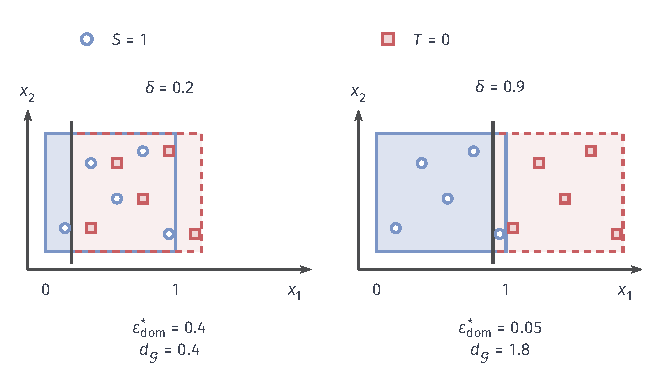
\includegraphics[width=113.404mm]{figures/02-foundations/02-learning-theory/tikz/learning-theory-domain-classifier/figure.pdf}
  \caption{域分类器的错误只对应输入散度项。源输入均匀分布于$[0,1]^2$，目标支持沿$x_1$平移$\delta$；圆点、方块的位置为教学构造，错误率由区域概率计算。$\mathcal H$含双向阈值与常值假设，域分类器类取$\mathcal G=\mathcal H\triangle\mathcal H$。其中$g=h_0\mathbin\oplus h_\delta$在左侧浅色带预测源域，$h_a(x)=\mathbb I\{x_1\geq a\}$；两域均等先验时，最小域错误为$(1-\delta)/2$，$d_{\mathcal G}=2\delta$。任务风险界还包含源风险及$\lambda=\inf_{h\in\mathcal H}(R_S(h)+R_T(h))$，不能只由域错误决定。}
 \label{fig:learning-domain-classifier}
\end{figure*}

分歧风险界允许标签规律以共同错误项$\lambda$进入结论，但无标签目标域样本不能直接估计这一项。若希望得到目标域超额期望风险可以趋于零的PAC保证，需要进一步规定源域标签为何仍能用于目标域。一种可以完整分析的设定是：两域共享条件标签分布，目标域出现的输入也能在源域观察到，而且两域输入频率的比例不会无限增大。

换测度积分公式与覆盖条件见
\BookSectionRef{sec:rv-change-measure}{第一卷“随机变量”章的“概率加权下的分布变换”一节}。
它们与迁移风险的联系在
\BookSectionRef{sec:future-data-law-object-map}{“数学基础与后续研究”章的“观测核与概率测度”一节}
中说明。本节在共享条件标签规律的设定下构造风险重加权，用$w(x)$表示目标输入分布相对于源输入分布的密度比。更一般地，$w$是满足
$\mathcal P_T^X(B)=\int_B w(x)\,\mathrm d\mathcal P_S^X(x)$的非负函数，其中$B$为任意可测输入集合。若$w(x)\leq\kappa$几乎处处成立，就有
\[
 \mathcal P_T^X(B)\leq\kappa\mathcal P_S^X(B).
\]
这既排除了源域完全遗漏的目标区域，也限制了源域对重要目标区域的低估程度。例如，目标域一半邮件属于某种类型、源域只有百分之一属于该类型时，任何适用的$\kappa$都至少为50。即使假设空间不变，这种稀少的源域观测也会增加学习难度。

在共享条件标签分布的前提下，目标域期望风险具有如下表达：
\begin{equation}
 R_T(h)=\mathbb E_{(x,y)\sim\mathcal P_S}
                 [w(x)\ell(h(x),y)].
 \label{eq:covariate-risk-identity}
\end{equation}
图~\ref{fig:learning-importance-weighting}把密度比落实到源域样本的贡献上。
目标域相对常见、源域相对稀少的输入获得较大权重；这些输入的标签仍然来自源域，
其有效性依赖共享条件标签机制，而非只依赖两条输入密度曲线。

\begin{figure}[htbp]
  \centering
  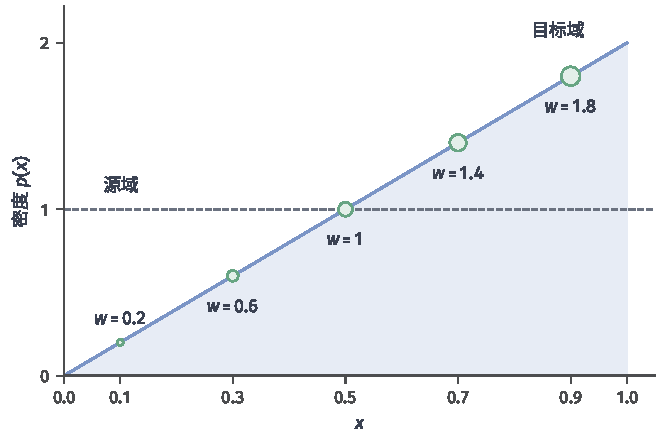
\includegraphics[width=\linewidth]{figures/02-foundations/02-learning-theory/matplotlib/learning-theory-importance-weighting/figure.pdf}
  \caption{重要性权重重新分配源样本的贡献。在$[0,1]$上构造源密度$p_S(x)=1$、
 目标密度$p_T(x)=2x$，二者均积分为1，因此$w(x)=2x$。
 五个源样本位置人为取为0.1、0.3、0.5、0.7、0.9，权重依次为0.2、0.6、1、1.4、1.8。
 圆点叠在目标密度上，面积与权重成正比，面积不表示局部样本数量。
 目标输入必须受到源输入覆盖；要使用风险恒等式，还需保持相同的条件标签分布。}
 \label{fig:learning-importance-weighting}
\end{figure}

等式来自把目标输入分布写为$w(x)\mathcal P_S^X$，而保持同一条件标签分布。它的理论作用是把不可直接观察的目标域标签损失，表示成源域上可以估计的期望。下面暂时假定$w$已知，以明确给出一个可学习的分布族；未知密度比所需的附加条件将在有限样本分析中讨论。

\subsection{基于假设空间的有限样本保证}
\label{sec:adaptation-classwide-bounds}

前一小节建立了两种总体层面的风险连接：分歧距离给出带有共同错误项的上界，重要性加权则在共享条件标签分布和覆盖条件下给出风险恒等式。接下来固定这些跨域联系，考察怎样同时控制整个假设空间中的经验风险与期望风险偏差。VC维适合控制二分类预测和分歧函数，Rademacher复杂度与参数范数则可处理加权实值损失。

\paragraph{分歧距离与VC维}

这个界尚未包含样本量，因为其中各项仍由真实分布定义。源域期望风险需要用带标签样本估计，分歧概率则可以用两域输入估计。两种估计都必须同时适用于全部假设或假设对，才能用于分析观察样本后选出的模型。

记$\widehat R_{S_S}(h)$为源样本$S_S$上的经验风险，$\widehat d$为把式~\eqref{eq:h-delta-h-divergence}中的两个概率替换为各自样本频率得到的经验散度。另记
\[
 \mathcal D_{\mathcal H}
 =\{x\mapsto\mathbb I\{h(x)\neq g(x)\}:h,g\in\mathcal H\}.
\]
它把“比较一对假设”转成一个取值为0或1的函数。若$c_{\mathcal H}(n,\delta)$给出源域经验风险与期望风险之差的统一上界，$c_{\mathcal D}(n,\delta)$给出分歧频率与真实分歧概率之差的统一上界，便有下面的有限样本结论。这里“统一”均指以概率至少$1-\delta$同时适用于相应函数空间的全部函数。

\begin{theorem}[有限样本的领域自适应期望风险界]
\label{thm:adaptation-finite-sample}
在定理~\ref{thm:domain-adaptation-bound}的条件下，以概率至少$1-\delta$，对全部$h\in\mathcal H$同时成立
\begin{equation}
 \begin{aligned}
 R_T(h)\leq{}&\widehat R_{S_S}(h)+\tfrac12\widehat d+\lambda\\
 &+c_{\mathcal H}(n_S,\delta/3)
  +c_{\mathcal D}(n_S,\delta/3)
  +c_{\mathcal D}(n_T,\delta/3).
 \end{aligned}
 \label{eq:adaptation-vc-risk}
\end{equation}
\end{theorem}
\begin{proof}
分别对源域分类损失、源域分歧函数和目标域分歧函数应用一致收敛保证。三项保证中至少一项失败的概率不超过$\delta/3+\delta/3+\delta/3=\delta$，这里不要求三项事件独立。在三项均成立时，对每对$h,g$，两域真实分歧概率之差与经验分歧频率之差的偏差不超过两个$c_{\mathcal D}$之和。取上确界后，有
\[
 \tfrac12d_{\mathcal H\triangle\mathcal H}
 \leq\tfrac12\widehat d
 +c_{\mathcal D}(n_S,\delta/3)+c_{\mathcal D}(n_T,\delta/3).
\]
再用$R_S(h)\leq\widehat R_{S_S}(h)+c_{\mathcal H}(n_S,\delta/3)$代入总体期望风险界即可。
\end{proof}

VC维在这里控制三项有限样本误差。若$\operatorname{VC}(\mathcal H)=d<\infty$，分类损失的预测数目受$\mathcal H$的生长函数控制。分歧函数由两个假设决定，所以在$m$个输入上的不同预测数目至多为$\Pi_{\mathcal H}(m)^2$。沿用式~\eqref{eq:vc-uniform-bound}的分析，当$1\leq d\leq n$时，两类$c$都可取为
\[
 O\!\left(\sqrt{\frac{d\log(2en/d)+\log(1/\delta)}{n}}\right).
\]
因此，为使每项抽样估计偏差不超过$\varepsilon$，充分的样本量具有
$O((d\log(1/\varepsilon)+\log(1/\delta))/\varepsilon^2)$的量级。无标签目标域样本在这个结论中用于估计分歧散度，并不用于估计$\lambda$。

参数数量可以通过VC维进入这个样本量要求。例如，$p$维输入上的仿射二分类假设空间具有$p+1$的VC维。对含$p$个参数、深度为$L$且满足第~\ref{chap:deep-learning-theory}章条件的ReLU网络，可使用$d=O(pL\log p)$的VC维上界，再代入上面的样本量公式。参数少通常有助于控制这部分抽样估计偏差，却不会自动减小$\lambda$。即使所有有限样本误差都趋于零，分布差异和共同预测条件仍然存在。因而式~\eqref{eq:adaptation-vc-risk}给出了目标域期望风险的上界，还不是整个分布族上的PAC可学习性刻画。

\paragraph{覆盖条件下的加权经验风险}
\label{sec:adaptation-coverage}

式~\eqref{eq:covariate-risk-identity}把目标域风险写成源域上的加权期望。若密度比已知且一致有界，便可以对整个有限假设空间同时估计这一加权风险，并由经验风险最小化得到目标域超额期望风险保证。

\begin{theorem}[已知密度比下的迁移样本量界]
\label{thm:covariate-finite-pac}
设$|\mathcal H|=N<\infty$，$\ell\in[0,1]$，两域共享条件标签分布，且已知密度比$0\leq w\leq\kappa$。给定$n$个独立源域样本，令
\[
 \hat R_w(h)=\frac1n\sum_{i=1}^n
          w(x_i)\ell(h(x_i),y_i),\qquad
 \widehat h\in\argmin_{h\in\mathcal H}\hat R_w(h).
\]
则以概率至少$1-\delta$，
\begin{equation}
 R_T(\widehat h)-R_{T,\mathcal H}^{\star}
 \leq\kappa\sqrt{\frac{2\log(2N/\delta)}{n}}.
 \label{eq:covariate-finite-excess}
\end{equation}
特别地，若$n\geq2\kappa^2\log(2N/\delta)/\varepsilon^2$，则目标域超额期望风险以概率至少$1-\delta$不超过$\varepsilon$。
\end{theorem}
\begin{proof}
对每个固定假设，$w(x_i)\ell(h(x_i),y_i)$取值在$[0,\kappa]$，其期望由式~\eqref{eq:covariate-risk-identity}给出。Hoeffding不等式与有限假设空间的概率求和保证，以概率至少$1-\delta$，全部假设同时满足
\[
 |R_T(h)-\hat R_w(h)|\leq
 a_n,\qquad a_n=\kappa\sqrt{\frac{\log(2N/\delta)}{2n}}.
\]
取目标域期望风险最小的$h^\star\in\mathcal H$，由经验最优性有
\[
 R_T(\widehat h)
 \leq\hat R_w(\widehat h)+a_n
 \leq\hat R_w(h^\star)+a_n
 \leq R_T(h^\star)+2a_n.
\]
代入$a_n$得到结论。
\end{proof}

这个定理回答了一个具体的可学习性问题：在共享标签机制、统一覆盖常数$\kappa$且密度比已知的分布族上，有限假设空间可以达到任意精度的目标域超额期望风险。证明用一个经验最小化规则说明这样的学习算法存在；核心依据是目标域期望风险能够被源域数据一致估计。给出的$\kappa^2$样本量依赖是充分条件，并不声称是最优依赖。

若密度比未知，仅有有限VC维还不够。需要额外说明能否从无标签两域样本估计$w$，以及估计误差如何下降。比如，在独立于上述带标签训练样本的数据上构造$0\leq\widehat w\leq\kappa$，记
\[
 b_w=\mathbb E_{x\sim\mathcal P_S^X}|\widehat w(x)-w(x)|.
\]
由于损失不超过1，对所有$h$都有
$|\mathbb E_S[\widehat w\ell(h(x),y)]-R_T(h)|\leq b_w$。
在保证该密度比误差的事件上重复证明，目标域超额期望风险上界增加$2b_w$，再合并该事件的失败概率。只有$b_w$也能在允许的分布族上一致趋于零，这一路径才继续给出PAC保证。密度比的可估计性是对分布族的要求，不能由预测假设空间的复杂度代替。

共享标签机制同样不能省去。若条件标签分布有所改变，令
\[
 b_{\mathrm{cond}}=\mathbb E_{x\sim\mathcal P_T^X}
 \operatorname{TV}\bigl(\mathcal P_S(\cdot\mid x),
                        \mathcal P_T(\cdot\mid x)\bigr),
\]
其中总变差距离$\operatorname{TV}$是两个概率分布对同一事件赋予概率的最大差。对$[0,1]$值损失，式~\eqref{eq:covariate-risk-identity}两端的差至多为$b_{\mathrm{cond}}$，上述超额期望风险界因此再增加$2b_{\mathrm{cond}}$。一个固定为正的残余项只能支持近似保证，不能保证任意小的目标域超额期望风险。

标签偏移需要另一种可识别条件。若源域两个类别的条件输入分布完全相同，那么无论目标域两个类别的比例怎样改变，无标签目标输入分布都相同，算法不能据此恢复类别比例。对于有限标签空间，若每个相关类别在源域具有正概率，带标签源数据才可能识别各类的条件输入分布；还需目标混合确实位于这些类条件分布的张成中，并要求它们线性独立，目标类别比例才具有点识别唯一性。有限样本下，仅有唯一性仍不够：恢复映射的最小奇异值必须在允许分布族上一致远离零，或等价地控制其条件数，同时还要给出源域各类的统一概率下界。否则微小估计误差会被任意放大。这说明不同偏移设定需要不同的跨域条件，不能共享一个仅由参数数量决定的可学习性判据。

\paragraph{参数范数与加权Rademacher复杂度}
\label{sec:transfer-norm-complexity}

VC维适合描述整个二分类假设空间的最坏情形。对高维线性模型或神经网络，这种上界可能很大，而学到的参数只处于一个较小的范数范围。第~\ref{chap:deep-learning-theory}章已经说明参数大小可以通过Rademacher复杂度控制期望风险；在迁移问题中，还需要追踪分布偏移怎样放大这一复杂度。

沿用前文的已知密度比设定。考虑$\mathbb R^p$上的线性预测$f_{\bm\theta}(\bm x)=\langle\bm\theta,\bm x\rangle$，其中$\|\bm\theta\|_2\leq B$、$\|\bm x\|_2\leq r$。损失$\ell(t,y)$对预测值$t$是$L$-Lipschitz的，即预测值相差$a$时，损失相差至多$L|a|$，并且损失取值在$[0,1]$中。范数限制约束模型输出对输入的敏感程度；密度比则决定每个源域输入对目标域期望风险的贡献。

\begin{theorem}[范数受限线性预测的迁移保证]
\label{thm:transfer-linear-norm}
在上述条件下，令$\widehat{\bm\theta}$最小化$n$个源域样本上的$\hat R_w$。以概率至少$1-\delta$，
\begin{equation}
 \begin{aligned}
 R_T(f_{\widehat{\bm\theta}})
 -\inf_{\|\bm\theta\|_2\leq B}R_T(f_{\bm\theta})
 \leq\frac{4\kappa LBr}{\sqrt n}
       +6\kappa\sqrt{\frac{\log(4/\delta)}{2n}}.
 \end{aligned}
 \label{eq:transfer-norm-excess}
\end{equation}
因此，存在普适常数$C$，当
$n\geq C\kappa^2((LBr)^2+\log(4/\delta))/\varepsilon^2$
时，目标域超额期望风险以概率至少$1-\delta$不超过$\varepsilon$。
\end{theorem}
\begin{proof}
记$\mathcal F_w$为加权损失函数空间。固定源域样本后，令$w_i=w(x_i)$，$\sigma_i$为相互独立的随机正负号。由Lipschitz收缩性质与欧氏范数的对偶关系，
\begin{align*}
 \widehat{\mathfrak R}_S(\mathcal F_w)
 &\leq\frac{LB}{n}\mathbb E_{\bm\sigma}
       \left\|\sum_{i=1}^n\sigma_iw_i\bm x_i\right\|_2\\
 &\leq\frac{LB}{n}\sqrt{\sum_{i=1}^n w_i^2\|\bm x_i\|_2^2}
 \leq\frac{\kappa LBr}{\sqrt n}.
\end{align*}
第二步使用Cauchy--Schwarz不等式；展开范数平方后，不同随机正负号的交叉项期望为零。收缩时可先减去每个样本上的$w_i\ell(0,y_i)$，这些与参数无关的项不改变Rademacher复杂度。

对加权损失$f\in\mathcal F_w$及其补函数$\kappa-f$，分别应用基于经验Rademacher复杂度的期望风险界。
两者都取值于$[0,\kappa]$；各分配$\delta/2$的失败概率，便能同时控制期望风险高于和低于经验风险的偏差，得到
\[
 \sup_{\|\bm\theta\|_2\leq B}
 |R_T(f_{\bm\theta})-\hat R_w(f_{\bm\theta})|
 \leq\frac{2\kappa LBr}{\sqrt n}
       +3\kappa\sqrt{\frac{\log(4/\delta)}{2n}}.
\]
经验最小化的目标域超额期望风险不超过这个统一偏差的两倍，证明完成。
\end{proof}

与参数计数相比，这个结论直接使用$B,r,L$，没有显式出现参数维数$p$。但“没有出现$p$”须在这些量不随$p$增大的前提下理解。例如，每个输入坐标都具有固定尺度时，输入范数$r$可能随$\sqrt p$增长，维度仍会间接进入样本量。增大覆盖常数$\kappa$也会增大所需源域样本量，这反映了稀少源域区域对目标域预测的重要性。

零一损失并不满足这里的Lipschitz条件。要用于分类，可以选择第~\ref{chap:deep-learning-theory}章介绍的间隔损失，以$L=1/\gamma$引入间隔$\gamma$，再用目标域间隔损失上界控制目标域分类期望风险。此时得到的是带有间隔条件的分类保证，不能直接改称相对于所有零一损失分类器的不可知PAC结论。对深度网络，也可用各层谱范数等量控制相应损失函数空间的Rademacher复杂度，再代入同样的跨域风险分析。一般损失下的分布差异与Rademacher分析可参见Mansour等的工作\scite{mansour2009adaptation}。

\subsection{基于输出的有限样本保证}
\label{sec:transfer-stability}
\label{sec:adaptation-output-bounds}

前一小节同时控制假设空间中的全部候选，所得结论适用于观察样本后选出的任意成员。本节改为分析算法实际输出：稳定性控制输出对训练样本的敏感程度，PAC--Bayes则评价训练结果附近的随机预测器。两条路线都只控制有限样本带来的误差，仍须保留相应的跨域条件和经验表现。

\paragraph{算法稳定性与可学习性}

参数范数限制整个可选假设空间，算法稳定性则描述训练数据变化时，算法实际输出的假设会改变多少。二者回答不同问题：参数较小不保证替换一个样本后参数变化较小；反过来，一个稳定算法也可能始终输出预测不准的固定假设。要从稳定性推出学习，还需要控制算法对经验目标的优化误差。

在已知密度比的协变量偏移设定下，这一关系可以直接由第~\ref{chap:convex-learning-and-stability}章得到。假设替换一个源域样本后，算法输出在任意输入标签对上的损失期望至多变化$\beta_n$，即算法对原损失具有均匀稳定性。乘上$w(x)\leq\kappa$后，加权损失的均匀稳定性参数至多为$\kappa\beta_n$。这里均匀稳定性的期望只针对算法内部随机性。

\begin{theorem}[稳定性条件下的迁移可学习性]
\label{thm:transfer-stability-learning}
设$\ell\in[0,1]$，两域共享条件标签分布，且已知密度比$0\leq w\leq\kappa$。算法$A$输出$\mathcal H$中的假设，对原损失具有均匀稳定性$\beta_n$，并满足
\[
 \mathbb E\!\left[\hat R_w(A(S))-
                  \inf_{h\in\mathcal H}\hat R_w(h)\right]
 \leq\rho_n.
\]
则
\begin{equation}
 \mathbb E[R_T(A(S))-R_{T,\mathcal H}^{\star}]
 \leq\kappa\beta_n+\rho_n.
 \label{eq:transfer-stability-excess}
\end{equation}
若$\kappa\beta_n+\rho_n$在允许的分布族上一致趋于零，则该设定PAC可学习。具体地，使$\kappa\beta_n+\rho_n\leq\varepsilon\delta$，便足以保证目标域超额期望风险以概率至少$1-\delta$不超过$\varepsilon$。
\end{theorem}
\begin{proof}
加权损失的均匀稳定性与式~\eqref{eq:covariate-risk-identity}给出
\[
 \mathbb E[R_T(A(S))-\hat R_w(A(S))]\leq\kappa\beta_n.
\]
对任意固定$h\in\mathcal H$，又有
\[
 \mathbb E\inf_{g\in\mathcal H}\hat R_w(g)
 \leq\mathbb E\hat R_w(h)=R_T(h).
\]
将目标域超额期望风险分解为期望风险与经验风险之差、经验优化误差以及最优经验风险与最优目标域期望风险之差，合并上述不等式并对$h$取下确界，得到期望结论。由于$A(S)\in\mathcal H$，目标域超额期望风险非负，对它使用Markov不等式即可得到所述概率保证。
\end{proof}

这里明确保留了两项条件。$\kappa\beta_n$控制目标域期望风险与加权经验风险之间的期望泛化差，$\rho_n$控制算法输出距离加权经验最优值还有多远。若$\beta_n\leq c/n$、$\rho_n\leq a/n$，上述充分条件为$n\geq(\kappa c+a)/(\varepsilon\delta)$。这个由期望经Markov不等式得到的样本量并不追求最优置信度依赖，却直接说明稳定性怎样支持迁移可学习性。

参数稳定性也由同一入口发挥作用。若损失关于参数是$G$-Lipschitz的，替换一个源域样本使输出参数的期望距离至多为$s_n$，则$\beta_n\leq Gs_n$，式~\eqref{eq:transfer-stability-excess}的右侧变为$\kappa Gs_n+\rho_n$。正则化或随机梯度下降的参数稳定性结论因而可以用于迁移分析，但必须核对其应用的是当前加权经验目标，以及相应的光滑性、凸性等条件。脱离共享标签机制与覆盖条件，即使参数完全不变，也不能保证目标域标签被正确预测。

\paragraph{参数分布与PAC--Bayes}
\label{sec:transfer-pac-bayes}

对随机训练或随机预测的模型，还可以通过参数分布描述复杂度。第~\ref{chap:deep-learning-theory}章的PAC--Bayes理论用后验分布偏离先验分布的程度控制源域期望风险与经验风险之差。迁移到目标域时，这个复杂度项仍然有效，但还需分析两个域上的预测分歧和共同错误怎样变化。

考虑二分类与零一损失。令$Q$为假设上的后验分布，Gibbs预测每次从$Q$抽取一个假设进行预测，其域$D$上的期望风险为$r_D(Q)=\mathbb E_{h\sim Q}R_D(h)$。独立抽取$h,g\sim Q$后，记$d_D(Q)$为二者在域$D$上的分歧概率，$e_D(Q)$为二者同时预测错误的概率，即
\begin{align*}
 d_D(Q)&=\mathbb E_{h,g\sim Q}\mathbb P_{x\sim\mathcal P_D^X}(h(x)\neq g(x)),\\
 e_D(Q)&=\mathbb E_{h,g\sim Q}\mathbb P_{(x,y)\sim\mathcal P_D}
                       (h(x)\neq y,\ g(x)\neq y).
\end{align*}
分歧可以用无标签输入观察，共同错误仍需要标签。这个区分使参数分布理论保留了迁移问题的信息边界，而不是把全部困难归入参数复杂度。

\begin{theorem}[参数分布的跨域期望风险界]
\label{thm:transfer-pac-bayes}
考虑二分类零一损失。设$n\geq1$，
$S_S\sim\mathcal P_S^n$，先验分布$P_0$与$S_S$独立。以概率至少$1-\delta$，
对所有$Q\ll P_0$同时有
\begin{equation}
 \begin{aligned}
 r_T(Q)\leq{}&\widehat r_{S_S}(Q)
 +\sqrt{\frac{D_{\mathrm{KL}}(Q\|P_0)+\log((n+1)/\delta)}{2n}}\\
 &+\tfrac12|d_T(Q)-d_S(Q)|+|e_T(Q)-e_S(Q)|,
 \end{aligned}
 \label{eq:transfer-pac-bayes}
\end{equation}
其中$\widehat r_{S_S}(Q)=\mathbb E_{h\sim Q}\widehat R_{S_S}(h)$。
\end{theorem}
\begin{proof}
固定$(x,y)$，令$p=\mathbb P_{h\sim Q}(h(x)\neq y)$。两个独立抽取的二分类假设分歧的概率为$2p(1-p)$，同时错误的概率为$p^2$。等式
$p=\tfrac12\cdot2p(1-p)+p^2$在域$D$上取期望后给出
\[
 r_D(Q)=\tfrac12d_D(Q)+e_D(Q).
\]
分别代入$D=T,S$并相减，可得
\[
 r_T(Q)\leq r_S(Q)+\tfrac12|d_T(Q)-d_S(Q)|+|e_T(Q)-e_S(Q)|.
\]
对$r_S(Q)$应用定理~\ref{thm:pac-bayes-bound}的PAC--Bayes上界，得到结论。
\end{proof}

这个推导采用Germain等研究中的分歧与共同错误分解\scite{germain2015adaptation}。
公式中的平方根项控制源域有限样本误差，另外两项控制同一后验预测分布在两域间的变化。
增加源域样本只能直接减小前一项；目标域共同错误差若没有结构条件控制，目标域无标签
样本仍不足以使整个上界趋于所需精度。

参数大小与参数分布在这里可以联系起来。例如，参数先验与后验分别为具有相同协方差$\sigma^2 I$的高斯分布，均值为$\bm\mu_0$和$\bm\mu$，则
\[
 D_{\mathrm{KL}}(Q\|P_0)=\frac{\|\bm\mu-\bm\mu_0\|_2^2}{2\sigma^2}.
\]
较小的参数位移可以降低这一复杂度项；增大$\sigma$虽也减小该表达式，却会改变随机预测并可能提高经验风险。源域经验风险与跨域残余项均已足够小时，给定一个与样本无关的上界$D_{\mathrm{KL}}(Q\|P_0)\leq K$后，
$n\geq[K+\log((n+1)/\delta)]/(2\varepsilon^2)$便足以使复杂度项不超过$\varepsilon$。
这是该期望风险上界给出的充分样本量条件，不是所有学习算法都必须满足的下界。若$Q$由数据选择，这个式子是对所选后验的风险证书；要得到预先给定的样本量，还需给出KL项的统一上界。

若把预训练模型用于构造先验，也必须保证该先验独立于这里用于计算经验风险的源域样本，或另行采用允许数据依赖先验的理论。

这一结论评价Gibbs预测的目标域期望风险，并不直接评价后验均值参数对应的确定性模型。与稳定性路线相比，PAC--Bayes控制参数分布相对于先验的复杂度，稳定性控制训练样本变化引起的输出变化。两者都可以刻画深度模型的泛化能力，但在迁移问题中都需要额外的跨域联系；没有任何一个参数复杂度量能够单独补出未观察到的目标标签。

\subsection{理论比较与适用边界}
\label{sec:adaptation-comparison}

领域自适应的各条路线都要区分跨域信息条件与有限样本控制。分歧距离路线用源域风险、输入分歧和共同错误项连接目标域风险；重要性加权路线依赖共享条件标签分布、输入覆盖和密度比；参数分布路线则对Gibbs预测器分解两域的分歧与共同错误。它们规定了不同的期望风险桥梁，不能仅因都出现复杂度项就视为同一种假设。

在风险桥梁固定以后，VC维、Rademacher复杂度和参数范数控制整个候选空间的估计偏差，算法稳定性控制实际训练输出对样本变化的反应，PAC--Bayes相对熵控制随机预测器相对于先验的复杂度。空间复杂度小不推出算法稳定，稳定算法也可能因为经验表现很差而无法学习；PAC--Bayes给出的Gibbs风险还不能直接改写成后验均值参数的风险。

更重要的是，有限样本项趋于零不等于迁移问题已经可学习。若$\lambda$、密度比估计误差、条件标签变化或共同错误差保持为正，已有观测仍不足以把目标域超额期望风险压到任意精度。领域自适应的PAC结论必须同时说明允许的分布族、可观察信息、跨域残余项和所采用的复杂度或稳定性条件。

\section{领域泛化的可学习性}
\label{sec:domain-generalization}

领域自适应可以利用目标域输入估计分布变化，领域泛化连这部分数据也没有。若目标环境可以任意选择，定理~\ref{thm:transfer-nonidentifiability}的反例仍然适用。因此，领域泛化理论必须明确新环境与训练环境的联系，以及“泛化成功”针对哪一种评价目标。

一种设定要求每个允许的目标域都保留共同预测机制，并限制它相对于训练域的覆盖关系。这能够导出对每个目标域的期望风险保证。另一种设定把环境本身看作随机对象，训练环境与未来环境来自同一环境分布；此时控制的是新环境上的平均期望风险。下面分别建立两类保证，再比较它们的评价对象、概率来源和适用边界。

\subsection{逐目标域保证}
\label{sec:dg-shared-mechanism}

多个训练域可以覆盖彼此遗漏的输入。设有$K$个源域分布$\mathcal P_1,\ldots,\mathcal P_K$，用
$\overline{\mathcal P}=K^{-1}\sum_{e=1}^K\mathcal P_e$表示它们的均匀混合分布。等概率选择一个训练域，再从该域抽取一个观测，就得到$\overline{\mathcal P}$的一个样本。若目标域的重要输入都在这个混合分布中有足够的出现机会，便有可能由训练域学习目标域需要的预测规律。

输入覆盖仍须与标签机制结合。对二分类问题，假定各训练域和允许的目标域共享
$\eta(x)=\mathbb P(y=1\mid x)$，并且贝叶斯分类器
$h^\star(x)=\mathbb I\{\eta(x)\geq1/2\}$属于$\mathcal H$。这比“所有训练域上存在同一个经验最优假设”强：它直接规定同一输入的条件标签规律在未来环境中仍然成立。

在这一条件下，可以比较同一假设相对于$h^\star$多犯的错误。若$h(x)=h^\star(x)$，条件超额错误概率为零；若两者不同，条件超额错误概率为$|2\eta(x)-1|$。因而对任一共享该机制的域$D$，
\begin{equation}
 R_D(h)-R_D(h^\star)
 =\mathbb E_{x\sim\mathcal P_D^X}
   [|2\eta(x)-1|\mathbb I\{h(x)\neq h^\star(x)\}].
 \label{eq:shared-bayes-excess}
\end{equation}
被平均的函数非负且在各域相同，输入覆盖条件就能够把训练域的超额期望风险转换为目标域的超额期望风险。

\begin{theorem}[共享标签机制下的领域泛化]
\label{thm:dg-shared-pac}
设$\mathcal H$为含$N<\infty$个假设的二分类假设空间，采用零一损失。训练域与全部允许的目标域共享$\eta$，相应贝叶斯分类器$h^\star$属于$\mathcal H$。若对每个允许的目标域与每个可测输入集合$B$都有
\[
 \mathcal P_T^X(B)\leq\kappa\overline{\mathcal P}^{X}(B),
\]
则从$\overline{\mathcal P}$独立抽取$m$个带标签样本并进行ERM，以概率至少$1-\delta$，对全部允许的目标域同时有
\begin{equation}
 R_T(\widehat h)-R_{T,\mathcal H}^{\star}
 \leq\kappa\sqrt{\frac{2\log(2N/\delta)}{m}}.
 \label{eq:dg-shared-pac}
\end{equation}
故$m\geq2\kappa^2\log(2N/\delta)/\varepsilon^2$是保证目标域超额期望风险不超过$\varepsilon$的充分样本量条件。

若进一步有$\eta(x)\in\{0,1\}$几乎处处成立，则任意与样本一致的假设都满足可实现PAC保证，只需
\[
 m\geq\frac{\kappa}{\varepsilon}
       \bigl(\log N+\log(1/\delta)\bigr).
\]
\end{theorem}
\begin{proof}
由式~\eqref{eq:shared-bayes-excess}与覆盖条件，对任意$h\in\mathcal H$，
\[
 R_T(h)-R_T(h^\star)
 \leq\kappa\bigl(R_{\overline{\mathcal P}}(h)
                  -R_{\overline{\mathcal P}}(h^\star)\bigr).
\]
$h^\star$在混合分布及各目标域中都是$\mathcal H$内最优假设。有限假设空间的不可知PAC样本量界给出
\[
 R_{\overline{\mathcal P}}(\widehat h)
 -R_{\overline{\mathcal P}}(h^\star)
 \leq\sqrt{\frac{2\log(2N/\delta)}{m}}.
\]
控制混合分布超额期望风险的同一个事件适用于全部目标域，因此得到同时保证。

在可实现情形，$R_D(h^\star)=0$。若某个假设在某个允许目标域上的期望风险大于$\varepsilon$，则它在混合分布上的期望风险必大于$\varepsilon/\kappa$。这样的固定假设与$m$个样本一致的概率至多为$\exp(-m\varepsilon/\kappa)$。对至多$N$个假设的失败概率求和，再令结果不超过$\delta$，得到第二个样本量条件。
\end{proof}

这个结论满足定义~\ref{def:targetwise-domain-generalization-pac}的逐目标域领域泛化要求，而且使用同一个高概率事件同时控制全部允许目标域，因而比定义中的逐目标域事件更强。算法不需要知道目标域的密度比，也不观察目标域样本，只需学习共享的最优分类器；覆盖条件保证它在源域混合分布上的错误不会在目标域被任意放大。这里的抽样模型是每次独立选择训练域并抽样，固定每域样本量的分层抽样应另行处理，不能直接把它宣称为混合分布的独立同分布样本。

有限性也可由更一般的复杂度控制替代。若$\mathcal H$在混合分布上满足偏差不超过$c_{\mathcal H}(m,\delta)$的一致收敛保证，同一证明给出目标域超额期望风险至多为$2\kappa c_{\mathcal H}(m,\delta)$。有限VC维由此提供领域泛化的一个充分条件；有界范数与合适损失下的Rademacher复杂度也可用于建立对应的源域估计保证。要把一般损失的源域超额期望风险转换到目标域，还须验证类似式~\eqref{eq:shared-bayes-excess}的非负条件超额损失关系。

这些条件也解释了不变性理论的作用。若已知表示$\Phi(x)$保留共同标签机制，可以在表示空间中要求共享条件标签分布与覆盖，再对$h\circ\Phi$进行上述分析。若表示由数据学习，就还需要证明训练环境能够识别这样的表示，并控制整个表示与预测器组合空间的复杂度。仅仅在有限训练环境中找到同一最优预测头，不能证明它在全部未来环境中仍然最优。不变风险最小化提出了寻找跨环境共同最优预测关系的思路\scite{arjovsky2019irm}。

在本章的理论问题中，关键是这种不变关系何时能够由训练环境确定。若训练环境变化不足，某个偶然相关的特征也可能在所有训练域上看起来稳定，却在目标域失效。IRM的风险分析揭示了这类限制\scite{rosenfeld2021irmrisk}。因此，不变性必须落实为关于允许环境、表示可识别性与假设空间的条件，不能仅用一个训练约束替代未来环境的假设。

\paragraph{表示充分性与近似误差}

逐目标域保证还需要区分有限样本造成的估计误差与表示本身造成的近似误差。固定一个已学习表示$\Phi$，记
$\mathcal H_\Phi=\{g\circ\Phi:g\in\mathcal G\}$。相对于目标域贝叶斯风险$R_T^{\mathrm{Bayes}}$，可分解为
\begin{equation}
 \begin{aligned}
 R_T(\widehat h)-R_T^{\mathrm{Bayes}}
 ={}&\left[R_T(\widehat h)-\inf_{h\in\mathcal H_\Phi}R_T(h)\right]\\
 &+\left[\inf_{h\in\mathcal H_\Phi}R_T(h)-R_T^{\mathrm{Bayes}}\right].
 \end{aligned}
 \label{eq:transfer-representation-bias}
\end{equation}
若只训练一个参数很少的预测头，可能更容易控制第一项，却无法保证第二项较小。例如，表示若把目标类别不同的输入映射到同一点，任何预测头都无法再区分它们。若表示与预测头在同一批数据上共同选择，也不能把表示事后当作独立固定对象而只计算预测头复杂度。共享机制、覆盖和复杂度控制只有与表示充分性结合，才能共同支持逐目标域保证。

\subsection{环境平均保证}
\label{sec:dg-random-environments}

对每个允许目标域都保留共同标签机制，是较强的要求。定义~\ref{def:environment-average-domain-generalization-pac}采用另一条路径：不指定每个目标域，而是假定环境来自同一个总体。例如，把不同用户视为不同环境，训练用户和未来用户都从同一个用户总体独立抽取。理论评价的对象便是未来随机用户上的平均期望风险。

令$\mathcal Q$为环境分布；从$\mathcal Q$抽取一次，得到一个输入标签联合分布$\mathcal P$。训练时独立抽取$K$个环境$\mathcal P_1,\ldots,\mathcal P_K$，再在每个环境内独立抽取$n$个样本$z_{e,i}=(x_{e,i},y_{e,i})$。给定各环境后，所有样本相互独立。对一个不随目标域重新训练的假设$h$，定义
\begin{equation}
 R_{\mathcal Q}(h)=\mathbb E_{\mathcal P\sim\mathcal Q}R_{\mathcal P}(h),
 \qquad
 \widehat R_{\mathcal S}(h)=\frac1{Kn}\sum_{e=1}^{K}\sum_{i=1}^{n}\ell(h,z_{e,i}).
 \label{eq:environment-average-risk}
\end{equation}
$\ell(h,z)$是$\ell(h(x),y)$的简写。$R_{\mathcal Q}$先在每个环境内平均损失，再对环境取平均；$\widehat R_{\mathcal S}$是从两层抽样得到的经验估计。

这一区别带来两类样本量。增加每个环境内的样本数$n$，能够更准确地评价已见环境；增加环境数$K$，才能更充分地了解环境之间的差异。固定$K$后无限增加$n$，并不等于观察了更多独立环境。

图~\ref{fig:learning-environment-sampling}比较了总观测数相同的两种扩充方式。
在原有环境中继续采样，会增加每行中的观测；另抽独立环境，则会增加行数。
环境平均风险还要对环境分布$\mathcal Q$取平均，所以这两种增加样本的方式不能互相替代。

\begin{figure*}[!htb]
  \centering
  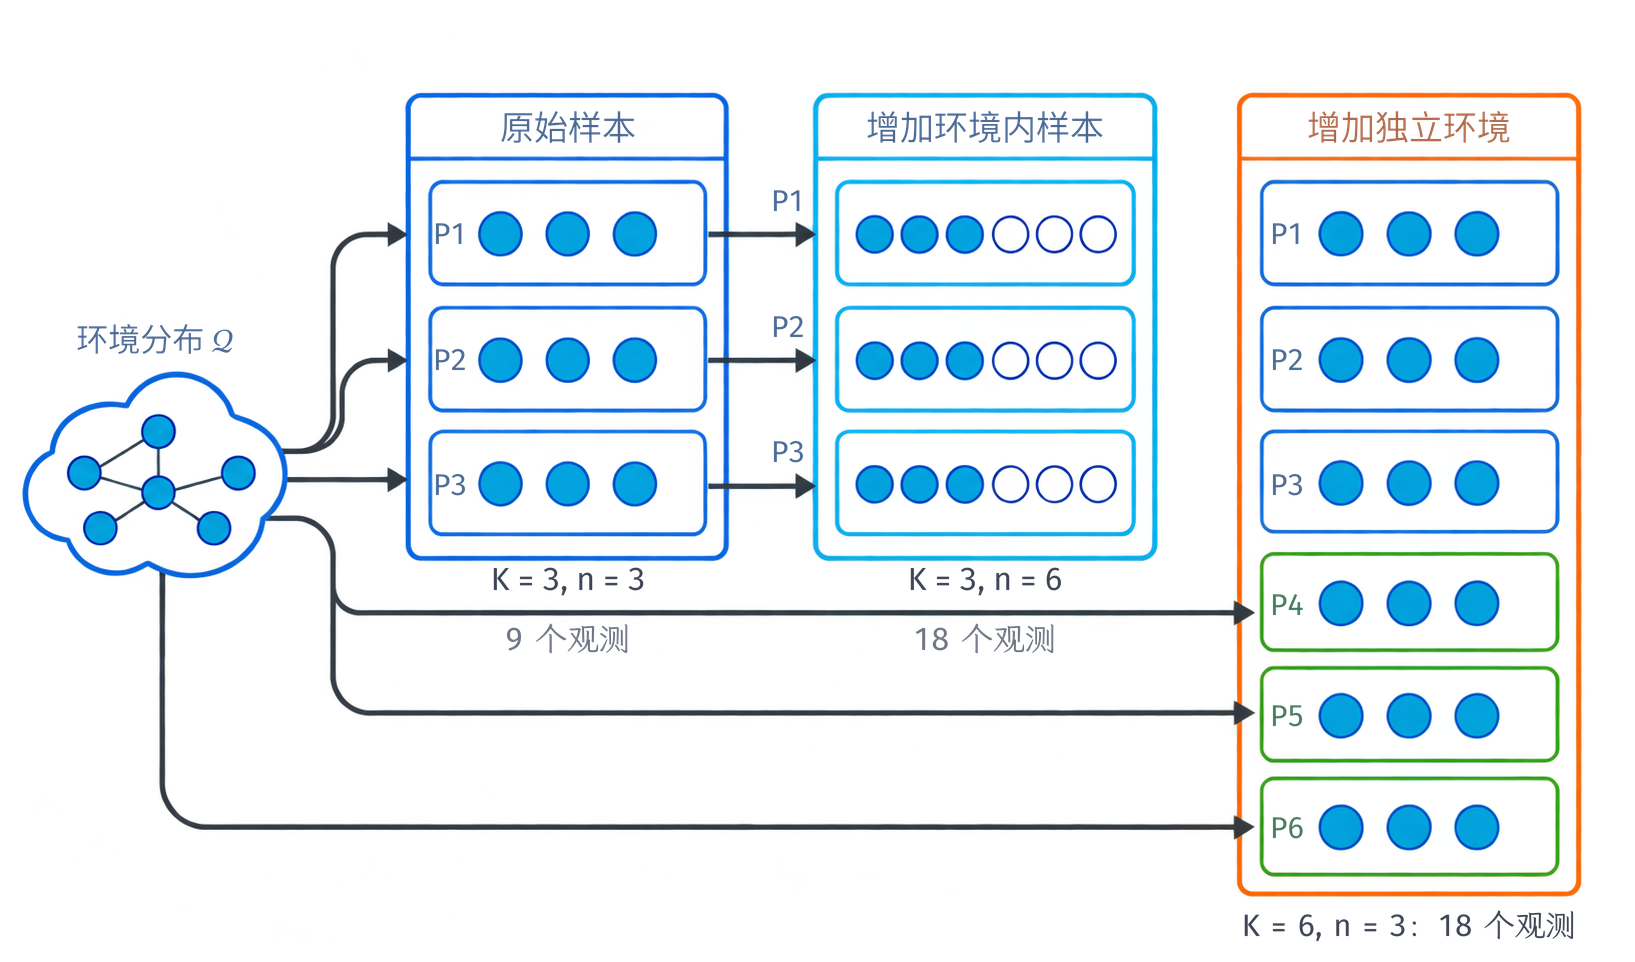
\includegraphics[width=164.600mm]{figures/02-foundations/02-learning-theory/generated/learning-theory-environment-sampling/figure.png}
  \caption{环境数量$K$与环境内样本数$n$对应不同的抽样层。每行边界代表一个环境，
 圆点代表其中的观测。左侧从同一环境分布$\mathcal Q$独立抽取3个环境，各取3个观测；
 中间的空心点表示在原有3个环境中继续抽取的观测，每个环境增至6个；右侧从$\mathcal Q$
 新抽取3个独立环境，每个环境仍取3个观测。
 中、右都有18个观测，只有右侧增加了独立环境数量。图中数量为教学构造，不对应实测数据。}
 \label{fig:learning-environment-sampling}
\end{figure*}

\begin{theorem}[随机环境中的一致收敛与可学习性]
\label{thm:dg-two-level-sample}
设$|\mathcal H|=N<\infty$、$\ell\in[0,1]$，数据按上述两层模型抽取。以概率至少$1-\delta$，对所有$h\in\mathcal H$同时有
\begin{equation}
 |R_{\mathcal Q}(h)-\widehat R_{\mathcal S}(h)|
 \leq\sqrt{\frac{\log(4N/\delta)}{2K}}
      +\sqrt{\frac{\log(4N/\delta)}{2Kn}}.
 \label{eq:dg-two-level-uniform}
\end{equation}
令$\widehat h$最小化$\widehat R_{\mathcal S}$，则其环境平均超额期望风险
$R_{\mathcal Q}(\widehat h)-\inf_{h\in\mathcal H}R_{\mathcal Q}(h)$
不超过上述右侧的两倍。特别地，令两项各不超过$\varepsilon/4$，即可得到定义~\ref{def:environment-average-domain-generalization-pac}中精度$\varepsilon$、置信度$1-\delta$的PAC保证。
\end{theorem}
\begin{proof}
在真实环境平均期望风险和经验风险之间插入已见环境的期望风险平均值：
\begin{align*}
 |R_{\mathcal Q}(h)-\widehat R_{\mathcal S}(h)|
 \leq{}&\left|R_{\mathcal Q}(h)-\frac1K\sum_{e=1}^K R_{\mathcal P_e}(h)\right|\\
 &+\left|\frac1K\sum_{e=1}^K R_{\mathcal P_e}(h)-\widehat R_{\mathcal S}(h)\right|.
\end{align*}
第一项包含$K$个独立环境，每个$R_{\mathcal P_e}(h)$都在$[0,1]$中。对固定$h$应用Hoeffding不等式，再对$N$个假设求和，以失败概率$\delta/2$得到第一项的统一上界。

第二项在给定全部$\mathcal P_e$后，是$Kn$个独立、有界但未必同分布的观测相对于各自期望的平均偏差。Hoeffding不等式仍然适用，再对$N$个假设求和，以条件失败概率$\delta/2$得到第二项上界。该保证对每组环境都成立，因此无条件失败概率也不超过$\delta/2$。合并两个事件得到一致收敛结论，ERM的超额期望风险再由两次偏差控制得到。
\end{proof}

由这个充分条件可取
\[
 K\geq\frac{8\log(4N/\delta)}{\varepsilon^2},\qquad
 Kn\geq\frac{8\log(4N/\delta)}{\varepsilon^2}.
\]
由于$n\geq1$，前者已经蕴含后者；这反映了当前对任意环境分布的最坏情形分析中，独立环境数量可能成为主要限制。并不是环境内的数据没有作用，而是没有进一步限制环境差异时，仅增加同一环境内的观测无法排除未见环境的变化。

对于无限假设空间，可以把证明中的两次有限计数替换成两层复杂度分析：环境层需要控制函数$\mathcal P\mapsto R_{\mathcal P}(h)$的复杂度，环境内需要控制损失函数$z\mapsto\ell(h,z)$的复杂度。参数数量、范数或Rademacher复杂度必须用于它们实际约束的那一层。若学习的是共享表示与各任务预测头，还需分别记录表示复杂度、预测头复杂度和任务数量；多任务表示学习与学习新任务的理论正是从这种区分中获得样本量结论\scite{maurer2016representation}。

这里的PAC比较对象是一个共同假设在随机新环境上的平均表现。它不保证每个环境的期望风险都小，也不与“知道目标环境后为它单独选择的最优假设”比较。若要学习一个能够根据目标域数据适应的算法，输出对象和比较基准都需要重新定义，不能沿用本定理而不作说明。

\paragraph{基于环境稳定性的算法保证}
\label{sec:dg-environment-stability}

前文的一致收敛证明同时控制整个假设空间。若希望分析实际算法，可以把第~\ref{chap:convex-learning-and-stability}章的稳定性理论用于环境层：将一个训练环境的全部样本换成另一个环境的样本，考察算法输出的预测损失变化。

记$D_e=(z_{e,1},\ldots,z_{e,n})$为第$e$个环境提供的数据块，$\mathcal S=(D_1,\ldots,D_K)$为全部训练数据。虽然同一块内的观测在不条件化环境时通常相关，不同的$D_e$仍然相互独立且同分布。对一个新块$D$，定义块损失
$L(h,D)=n^{-1}\sum_{i=1}^n\ell(h,z_i)$。它的总体期望正好是$R_{\mathcal Q}(h)$，因此可以把每个环境块当作稳定性分析的一个观测单位。

\begin{definition}[环境均匀稳定性]
\label{def:environment-stability}
设$A$接收$K$个环境数据块。若对任意仅在一个数据块上不同的$\mathcal S,\mathcal S'$，以及任意测试观测$z$，均有
\[
 \left|\mathbb E_A\ell(A(\mathcal S),z)
       -\mathbb E_A\ell(A(\mathcal S'),z)\right|\leq\gamma_K,
\]
则称$A$具有参数为$\gamma_K$的环境均匀稳定性。
\end{definition}

\begin{theorem}[环境稳定性与平均可学习性]
\label{thm:dg-environment-stability}
在定理~\ref{thm:dg-two-level-sample}的抽样模型下，允许$\mathcal H$无限。若$A$输出$\mathcal H$中的假设，具有环境均匀稳定性$\gamma_K$，且
\[
 \mathbb E\!\left[\widehat R_{\mathcal S}(A(\mathcal S))-
                  \inf_{h\in\mathcal H}\widehat R_{\mathcal S}(h)\right]\leq\rho_{K,n},
\]
则
\[
 \mathbb E\!\left[R_{\mathcal Q}(A(\mathcal S))-
                  \inf_{h\in\mathcal H}R_{\mathcal Q}(h)\right]
 \leq\gamma_K+\rho_{K,n}.
\]
若对任意$\varepsilon,\delta\in(0,1)$都存在门槛$k_0,m_0$，使所有允许的
$\mathcal Q$及所有满足$K\geq k_0$、$Kn\geq m_0$的抽样方案都有
$\gamma_K+\rho_{K,n}\leq\varepsilon\delta$，则满足
定义~\ref{def:environment-average-domain-generalization-pac}中的环境平均PAC要求。
这是一条同时对$K$与$Kn$量化的条件；只沿某条令$K,n\to\infty$的增长路径收敛并不足够。
\end{theorem}
\begin{proof}
环境均匀稳定性也控制块损失$L$的变化，因为对块内每个观测的损失变化取平均仍不超过$\gamma_K$。不同数据块独立同分布，故均匀稳定性定理给出
\[
 \mathbb E[R_{\mathcal Q}(A(\mathcal S))-\widehat R_{\mathcal S}(A(\mathcal S))]\leq\gamma_K.
\]
对任意固定$h$，$\mathbb E\widehat R_{\mathcal S}(h)=R_{\mathcal Q}(h)$，从而
$\mathbb E\inf_h\widehat R_{\mathcal S}(h)\leq\inf_hR_{\mathcal Q}(h)$。
加入经验优化误差即得期望结论，再对非负的超额期望风险应用Markov不等式。
\end{proof}

普通样本稳定性与环境稳定性之间也有明确联系。如果替换任意单个观测的均匀稳定性参数为$\beta_{Kn}$，逐个替换一个块内的$n$个观测并累加损失变化，就得到
$\gamma_K\leq n\beta_{Kn}$。例如，$\beta_{Kn}=O(1/(Kn))$只能直接推出$\gamma_K=O(1/K)$；增加每个环境内的样本，并不会在这个推导中消除有限环境数量的影响。若替换一个环境块引起的参数期望距离至多为$s_{K,n}$，损失又是$G$-Lipschitz的，则同样可取$\gamma_K\leq Gs_{K,n}$。

\subsection{两类保证的比较与适用边界}
\label{sec:dg-guarantee-comparison}

逐目标域保证先固定一个允许目标域，再要求训练得到的同一输出在该域上接近相应比较基准。共享标签机制与覆盖条件说明源域混合风险为何能够约束这个目标域；若同一个高概率事件覆盖全部允许目标域，还可以得到比逐域定义更强的同时保证。环境平均保证则把未来环境视为从$\mathcal Q$抽取的随机对象，评价的是共同假设在环境总体上的平均风险。它允许某些具体环境表现较差，不能自动改写成对每个未见环境都有效。

两类保证中的样本量也承担不同作用。逐目标域路线依赖训练数据是否覆盖目标域所需的输入和标签机制；环境平均路线则必须区分独立环境数量$K$与每个环境内的样本数$n$。增加$n$可以更准确地评价已见环境，却不能替代新的独立环境。相应地，普通样本稳定性控制环境内部的数据变化，环境稳定性控制替换整个环境后的算法变化，二者不能只因都称为稳定性便互换。

参数数量、范数和表示复杂度可以控制候选空间的估计误差，参数稳定性可以控制算法对训练数据或训练环境的敏感程度，但这些量都不能单独提供跨域联系。逐目标域保证仍需共享机制、覆盖和表示充分性，环境平均保证仍需训练环境与未来环境来自同一环境分布。评价基准、跨域条件与有限样本控制共同决定结论能够推广到哪里。

\Needspace{8\baselineskip}
\section{本章小结}
\label{sec:transfer-learning-summary}

训练与使用分布不同时，目标域可学习性的首要条件是可观察的训练信息与目标域标签保持
足够联系。即使假设空间只有两个成员，缺少覆盖或标签联系也可能使目标预测无法识别。
因此，参数数量、范数与稳定性不能单独刻画迁移是否成功；它们控制有限样本学习的困难，
跨域假设则决定这些信息能否用于目标域。

领域自适应允许观察目标域数据，但无标签数据只能直接说明输入分布。分歧距离和共同
错误项把源域与目标域期望风险联系起来；协变量偏移配合覆盖条件，则能把目标域评价
写成源域上的加权评价。在明确密度比是否已知、能否估计以及损失条件之后，VC维、
Rademacher复杂度、PAC--Bayes与稳定性才可给出相应的有限样本保证。一个仍含有不可控
跨域残余项的期望风险上界，不能直接称为整个分布族上的PAC可学习性刻画。

领域泛化进一步取消训练时的目标域样本。定义~\ref{def:targetwise-domain-generalization-pac}逐一固定允许的目标域，共享标签机制与覆盖为这种保证提供一条充分路径；定义~\ref{def:environment-average-domain-generalization-pac}把训练环境与未来环境视为来自同一环境分布的独立抽样，控制对新环境的平均表现。两者的评价对象和概率来源不同。增加每个环境内的观测数量，通常不能代替增加独立训练环境的数量；环境稳定性也必须与经验优化要求结合。

本章及本部分的可学习性结论只回答：在给定观测、损失、比较空间和允许分布族后，是否
存在算法，使任意误差容限$\varepsilon$与失败概率容限$\delta$都对应一个统一的有限样本量
门槛，并对分布族中的每个允许分布以至少$1-\delta$的概率使期望风险落入相应误差范围。
它不判断所选损失是否覆盖真实
使用后果，也不判断比较基准对应的表现是否可接受；对分布族之外的数据、系统组合或
部署条件变化后的表现也没有自动保证。预训练、持续偏移与有限目标监督所提出的研究问题
已在第~\ref{sec:learning-theory-research-content}节集中说明；处理这些问题时，仍须先把可见信息、
分布变化和比较对象写入学习问题。这些对象尚未明确时，更小的复杂度上界不能补足结论。

\paragraph{延伸阅读}
Ben-David等的领域自适应理论与不可学习性结果适合配合阅读。期望风险上界说明分布
差异和共同预测能力各自起什么作用，不可能性结果则说明缺少这些联系时，为什么更多
源域数据或无标签目标域数据仍可能不足。对照两类结论，可以避免把某个上界中的
复杂度项下降误认为整个迁移问题已经可学习\scite{bendavid2010adaptation,bendavid2010impossibility}。

若希望继续研究参数分布如何参与跨域分析，可阅读Germain等的PAC--Bayes领域自适应
分解，区分源域抽样误差、预测分歧变化与共同错误变化。这个视角也有助于检查哪些项
能由无标签样本估计，哪些项仍需关于标签机制的假设\scite{germain2015adaptation}。

Maurer、Pontil与Romera-Paredes对多任务表示学习的分析，适合继续研究环境数量、
环境内样本量与表示复杂度怎样共同影响学习。阅读时应保留其任务抽样与共享表示条件，
避免将对环境分布平均的保证解释成对任意新环境都成立的保证\scite{maurer2016representation}。
